% Created 2016-02-29 Mon 15:13
% Intended LaTeX compiler: pdflatex
\documentclass[11pt]{article}
\usepackage[utf8]{inputenc}
\usepackage[T1]{fontenc}
\usepackage{graphicx}
\usepackage{grffile}
\usepackage{longtable}
\usepackage{wrapfig}
\usepackage{rotating}
\usepackage[normalem]{ulem}
\usepackage{amsmath}
\usepackage{textcomp}
\usepackage{amssymb}
\usepackage{capt-of}
\usepackage{hyperref}
\usepackage{minted}
\usepackage{pdfpages}
\author{bachir el khadir}
\date{\today}
\title{}
\hypersetup{
 pdfauthor={bachir el khadir},
 pdftitle={},
 pdfkeywords={},
 pdfsubject={},
 pdfcreator={Emacs 25.1.50.1 (Org mode )}, 
 pdflang={English}}
\begin{document}

\begin{HTML}

\label{orgspecialblock1}

\end{HTML}




\section{Discover Gravitational Wves in Your Room}
\label{sec:orgheadline1}


\textbf{1.1)}

Loading the Data

\begin{minted}[frame=lines,linenos=true]{r}
ts <- read.table('LIGO.Hanford.Data.txt')
ts.theory <- read.table('LIGO.Hanford.Theory.txt')
names(ts) <- c("t", "y")
names(ts.theory) <- c("t", "y")
N <- length(ts$y)
\end{minted}




Calculate the matrix \(C\)

\begin{minted}[frame=lines,linenos=true]{r}
C <- matrix(sqrt(1 / N), N, N)
for(j in 2:N) 
    for(k in 1:N)
        C[j, k] = sqrt(2 / T) * cos(pi * (2*k-1) * (j - 1) / (2*N) )
\end{minted}


Solve the lasso, and use 10-fold cross-validation to choose \(\lambda\)

\begin{minted}[frame=lines,linenos=true]{r}
library(glmnet)
lasso.model <- cv.glmnet(C, ts$y, alpha=1, nfolds=10, intercept=F)
w.hat <- coef(lasso.model, s='lambda.1se')[-1]
w.inverse <- solve(C, ts$y)
lasso.model$lambda.1se
\end{minted}




\begin{verbatim}
lambda.1se =  0.003515
\end{verbatim}



\includegraphics[width=.9\linewidth]{comparesignals.png}


\includegraphics[width=.9\linewidth]{comparesignalsspec.png}

The lasso behaves like a high-pass filter, it eliminates the lowest frequencies.

\textbf{1.2)}

The denoised signal is \(\tilde y + C \tilde w = \Psi \tilde \beta\)
\begin{minted}[frame=lines,linenos=true]{r}
psi <- cbind(diag(N), C)
lasso.model2 <- cv.glmnet(psi, ts$y, alpha=1, nfolds=10, intercept=F)
beta.tilde <- coef(lasso.model2, s='lambda.1se')[-1]
y.tilde <- psi %*% beta.tilde
lasso.model2$lambda.1se
\end{minted}


\begin{verbatim}
lambda.1se =  0.004436
\end{verbatim}


\includegraphics[width=.9\linewidth]{comparesignals2.png}

\begin{itemize}
\item The first method eliminates large spikes (low frequencies), but is sensitive to recurrent small variations.
\item The second method is more robust to small variations but is sensitive to large outliers.
\end{itemize}

The second method is more meaningful because it looks for sparsity in time and frequency domain, and there is no reason for the noise to be added in one domain and not the other.


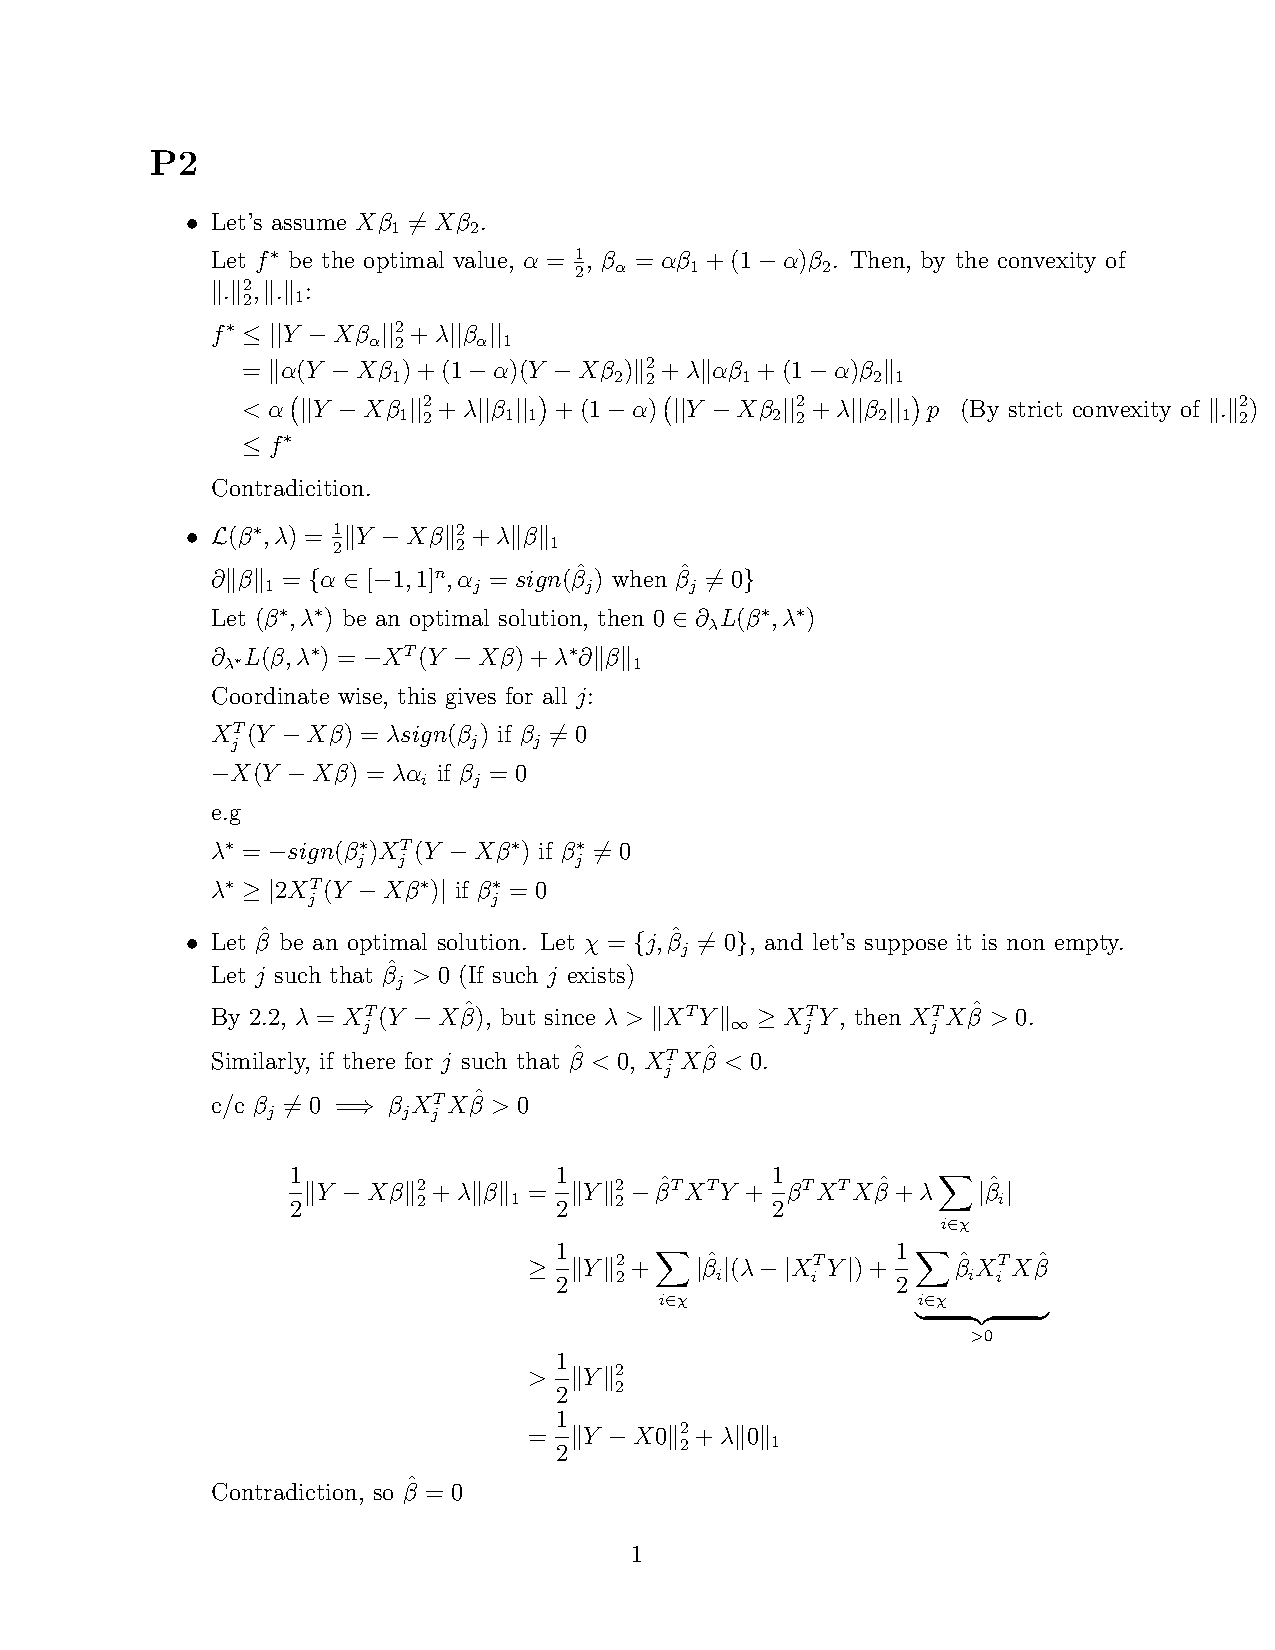
\includepdf[pages=-]{q2.pdf}
\end{document}